\documentclass[11pt,a4paper]{article}
\usepackage[margin=22mm]{geometry}
\usepackage[T1]{fontenc}
\usepackage{lmodern,amsmath,amssymb,booktabs,graphicx,hyperref,array,fancyhdr}
\hypersetup{colorlinks=true,urlcolor=blue,linkcolor=black,citecolor=black}
\setlength{\parindent}{0pt}\setlength{\parskip}{5pt}
\pagestyle{fancy}\fancyhf{}\lhead{Tree-Type Neural Networks: Continuation}\rhead{2025EEA3026}\cfoot{\thepage}
\newcommand{\fig}[2]{\begin{center}\includegraphics[width=.86\linewidth]{figures/#1}\par\small #2\end{center}}
\begin{document}
\begin{titlepage}
\centering
\vspace*{2mm}
{\Large\bfseries ASSIGNMENT 5}\\[18mm]
{\large\bfseries MACHINE LEARNING AND OPTIMIZATION (ELL7285)}\\[9mm]
{\Large\bfseries TREE-TYPE NEURAL NETWORKS}\\[4mm]
{\large Augmentation, ensembles, bias--variance and loss geometry\\on CIFAR-10 and Cats vs Dogs}\\[3mm]
{\normalsize (continuation of Assignment 4)}\\[16mm]
{\bfseries Submitted by}\\[4mm]
Durgesh Singh (2025EEA3026)\\[14mm]
{\bfseries Under the guidance of}\\[2mm]
Prof.~Jayadeva\\[16mm]
{\itshape In partial fulfilment of the requirements for the award of the degree of}\\[2mm]
{\bfseries Master of Technology}\\[10mm]

\includegraphics[width=42mm]{figures/iitd_logo.png}\\[10mm]
Department of Electrical Engineering\\[2mm]
{\bfseries Indian Institute of Technology Delhi}\\[4mm]
{\bfseries October 2026}
\end{titlepage}
\setcounter{page}{1}
\begin{abstract}
This continuation of Assignment 4 retains the neural correction-tree construction (frozen MobileNetV3-Small features, MLP nodes and a constrained readout refit) and studies input augmentation on Cats vs Dogs and CIFAR-10 across 696 training runs. (i) Augmentation coexists with zero fitted training error and, in clean root-only width sweeps, lowers test error by 0.15--0.50 points where a four-copies exposure control does not; under 15\% label noise it is harmful at small widths. Noisy width sweeps show an error peak followed by recovery, but not a complete decrease--increase--decrease curve. (ii) A seven-member hard-voting ensemble with diverse augmentation banks reaches 97.94\% on Cats vs Dogs and 89.91\% on CIFAR-10, $+0.13$ and $+0.70$ points over the unaugmented ensemble. The CIFAR-10 gain survives a paired bootstrap and a change of tie rule, and comes mainly from stronger members and fewer shared errors rather than more disagreement; neither ensemble beats a single wider tree from Assignment 4. (iii) More original samples reduce the bias-related term and the variance on CIFAR-10, while longer per-node training raises both probability variance and replicate label disagreement. (iv) In normalized two-dimensional slices, augmented fits sit in steeper, not flatter, basins. The proposed persistence-weighted correction rule shows no convincing benefit; these negative findings are retained.
\end{abstract}

\textbf{GitHub repository:} \texttt{https://github.com/dugu01/Tree\_Network\_2025EEA3026}

\section{Architecture and fitting}
A frozen ImageNet-pretrained MobileNetV3-Small feature extractor produces $z\in\mathbb R^{576}$. Its 927,008 parameters are shared by all nodes and ensemble members. Each node has a one-hidden-layer ReLU MLP, with hidden width $h$. For binary tree node $v$, using the earlier report's notation,
\begin{align*}
 r_v(z)&=\operatorname{ReLU}(W_vz+c_v), & s_v(z)&=u_v^\top r_v(z)+b_v,\\
 F_v(z)&=s_v(z)+a_vH_A(z)-d_vH_B(z), & H_v(z)&=\mathbf1[F_v(z)\geq0],
\end{align*}
with $a_v,d_v\geq0$ and children $A,B$. The children learn correction decisions for the parent's false negatives and false positives. Cats vs Dogs uses one binary tree. CIFAR-10 uses ten one-versus-rest trees; the largest root score gives the class. Thus one CIFAR-10 ensemble member is a complete ten-class predictor, not one binary root.

Local MLPs minimize class-balanced binary cross-entropy with Adam (learning rate $10^{-3}$, batch size 512, no weight decay). Maximum correction depth is two. After child construction, an L-BFGS-B readout refit minimizes uniform BCE plus an $L_2$ penalty of $10^{-6}$, with nonnegative correction coefficients. A refit is accepted only if the pair (training errors, BCE) improves lexicographically, including a float32 check. Early stopping is disabled for the prescribed epoch budgets. A root that already classifies its training data correctly need not grow children.

\textbf{Interpretation.} Width and retained node count both determine capacity. A nominal ``tree'' can finish as a root-only predictor; results below explicitly distinguish these cases. The pretrained representation makes this a transfer-learning experiment, not training an image model from scratch.

\section{Data and input augmentation}
\begin{center}\begin{tabular}{lrrr}\toprule
Dataset & Original training images & Validation & Test\\\midrule
Cats vs Dogs &17,476&3,745&3,745\\
CIFAR-10 &45,000&5,000&10,000\\\bottomrule
\end{tabular}\end{center}
Original cleaned splits are retained. Standardization is fitted only on selected original training features. Augmentation is applied to RGB images \emph{before} the frozen encoder. CIFAR-10 uses a reflected-padding random crop (32 pixels, padding 4), horizontal flip and mild colour jitter. Cats vs Dogs uses a random resized crop to 224 pixels (area scale 0.8--1.0, aspect ratio 0.9--1.1), flip and the same jitter (brightness/contrast/saturation 0.1, hue 0.02).

\subsection{Experimental controls and provenance}
Each augmented fit uses the original plus three fixed transformed views per image. Nine cached training views provide three distinct augmentation banks. Two further views per training image are held out as invariance probes; they are correlated with training images and are not independent test samples. These are finite cached augmentations, not newly resampled transforms at every epoch.

The controls are: no augmentation; four copies of each original (exposure control); uniform augmentation; and persistence-weighted augmentation. Repetition matches root input multiplicity but not necessarily total child updates, because correction subsets and tree sizes adapt. A separate condition assigns 15\% label noise in the full training pool; every view inherits its original's assigned label. A selected subset's actual corruption fraction may differ from exactly 15\%. Validation and test labels remain clean.

\begin{center}\small\begin{tabular}{p{34mm}p{116mm}}\toprule
Study & Design\\\midrule
Capacity & 25\% of original training pool; 100 epochs/node; seeds 17, 29, 43; clean/15\% noise; root-only widths 4--256, selected depth-two widths; Cats vs Dogs refined down to width 1.\\
Ensembles & Full training pool; width 4, depth two, 100 epochs/node; four families with seven seeds each; committees of 1, 3, 5, 7.\\
Bias--variance & Width 4; 10\%, 25\%, 50\% original samples; three data seeds crossed with two initialization seeds; 10, 30, 100 epochs/node; no augmentation/augmentation.\\
Epoch trajectories & Root-only width 32; two seeds; clean/noisy and unaugmented/augmented; saved checkpoints through 500 epochs; 25\% training pool.\\
Landscape & Clean width-4 depth-two fits, seed 17; no augmentation/augmentation; three direction pairs; $15\times15$ grids, radius 0.3; 512 training and validation samples.\\\bottomrule
\end{tabular}\end{center}

There are 696 completed run records: 408 Cats vs Dogs and 288 CIFAR-10. Twenty-four Cats vs Dogs refinement records repeat earlier configurations with identical prediction hashes. They are excluded from independent replicate statistics, leaving 672 unique configurations including pilots. The repeated runs provide reproducibility checks, not extra seeds.

The experiment settings and primary comparison (seven-member diverse augmentation versus seven-member no augmentation) were frozen before the new test evaluation. Every planned checkpoint was evaluated; no best test seed or best voting subset was selected. The original assignment had already used these test splits: the lock prevents further tuning in this continuation, but does not make them historically unseen benchmarks.

\textbf{Audit.} The saved labels and predictions allow independent recalculation of all 696 validation/test classification-error counts and log losses (within $10^{-4}$ for float32 export), canonical ensemble voting and the bias--variance identity. Prediction/label hashes and checkpoint-hash declarations agree with the plans and test locks. Raw images, full feature banks and model checkpoints are not in the evidence bundles, so this audit does not independently rerun training or inference.

\begin{center}
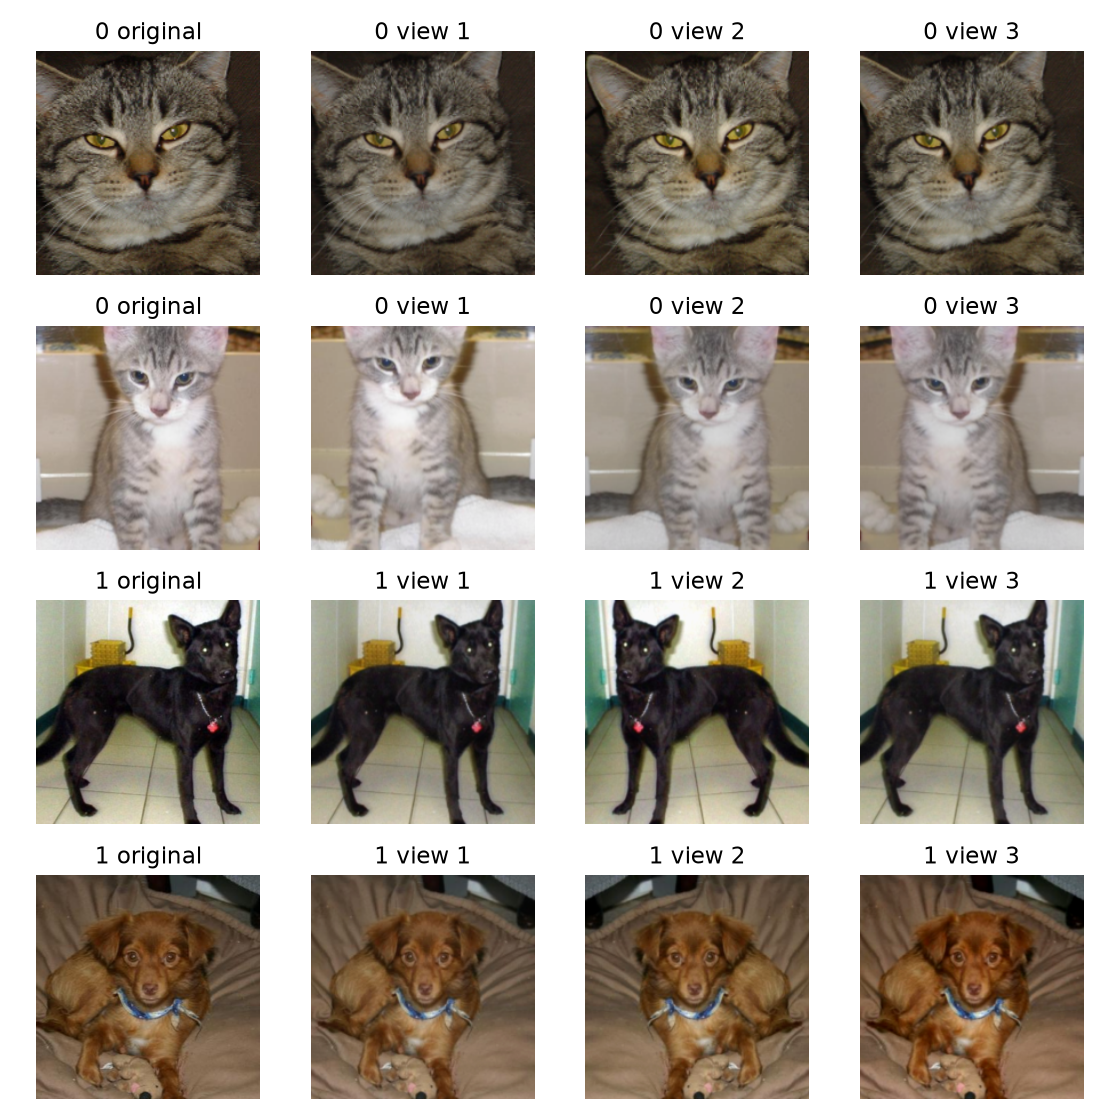
\includegraphics[height=49mm]{figures/catsdogs_augmentation.png}\hspace{8mm}
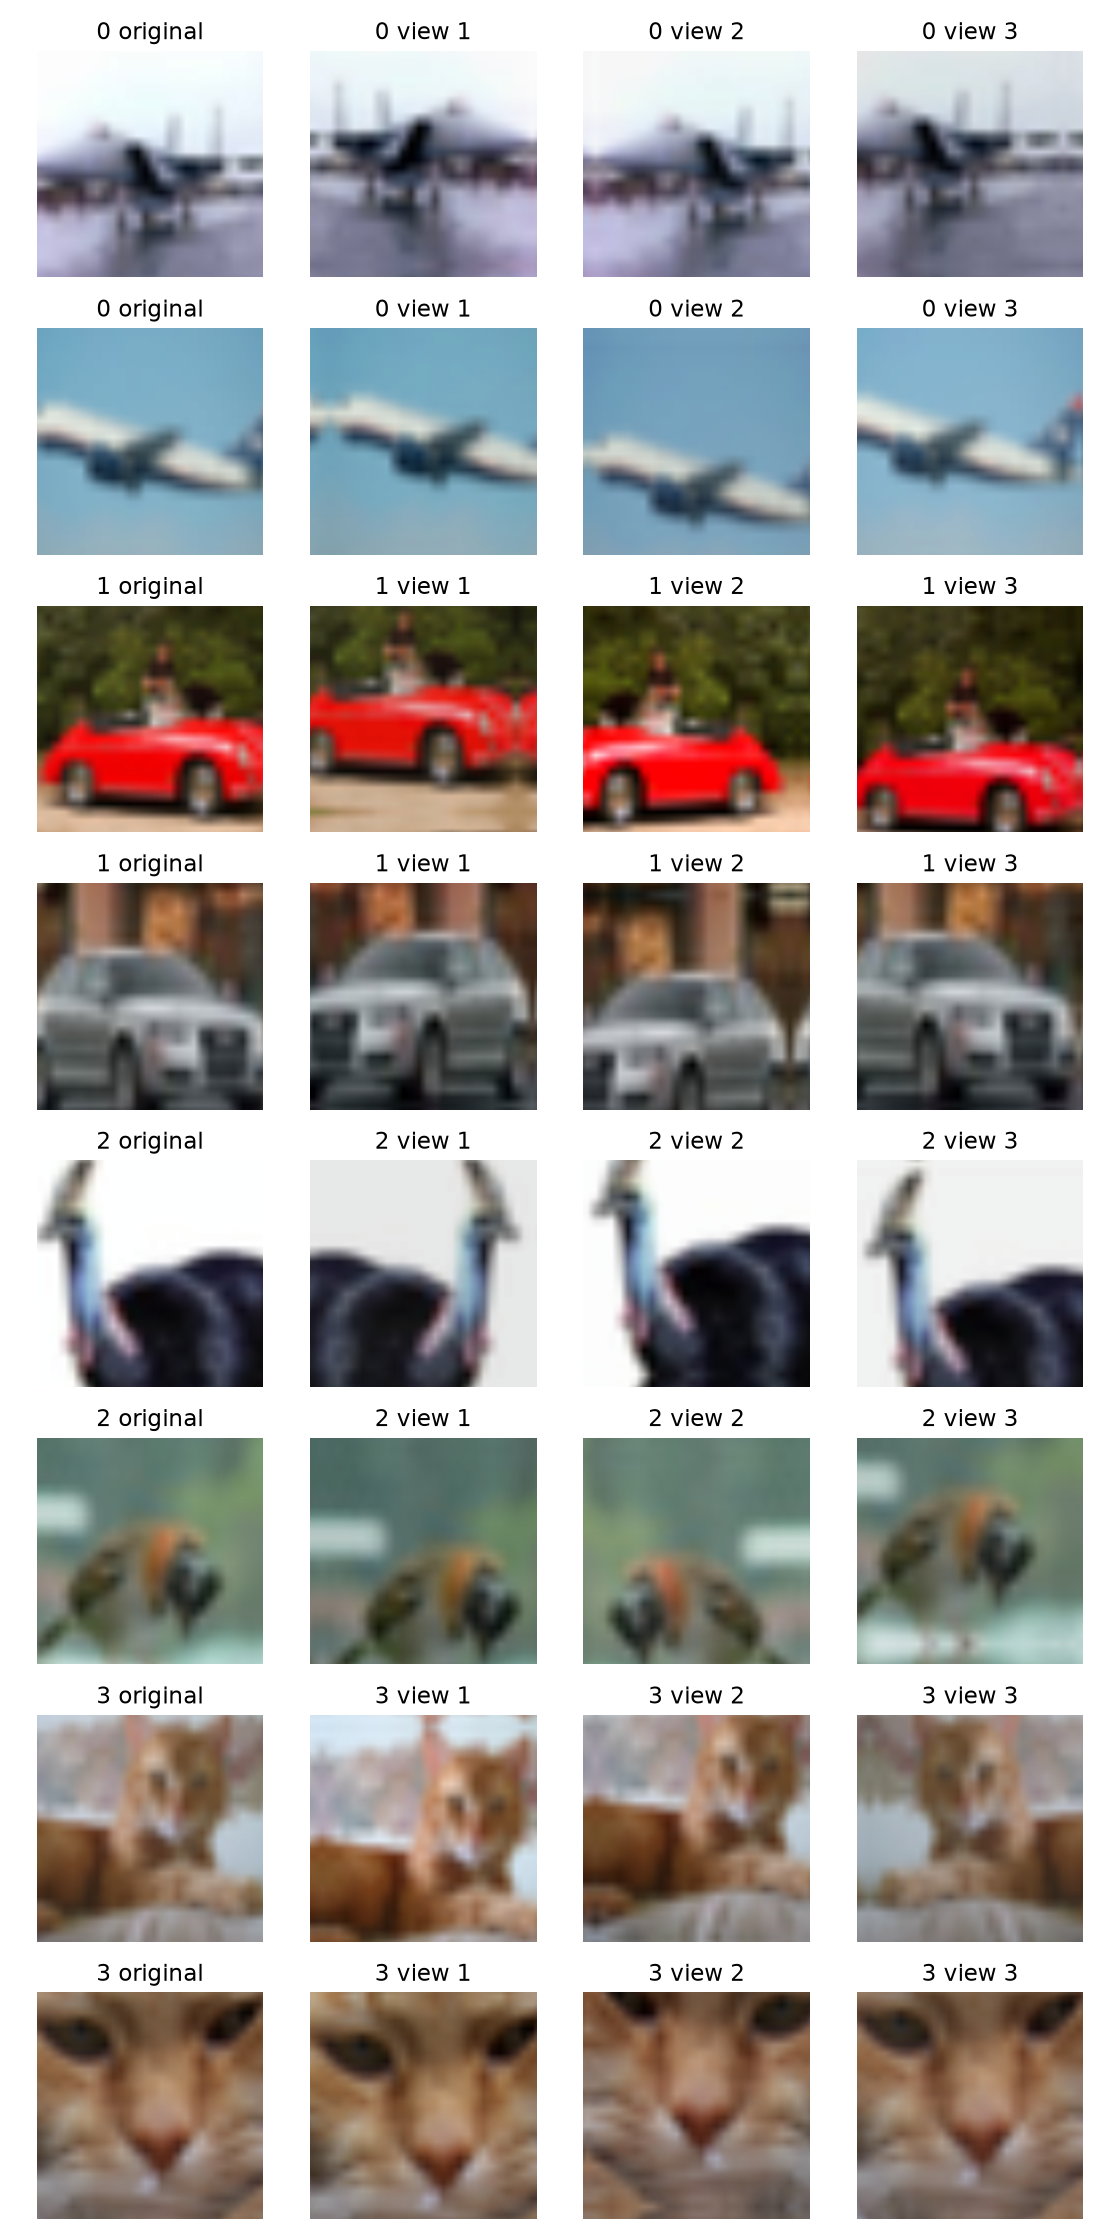
\includegraphics[height=49mm]{figures/cifar10_augmentation.png}\\
\small Audit contact sheets: originals and three views. Full-resolution images are supplied in the package.
\end{center}
The inspected examples retain plausible class identity despite cropping, reflection and colour variation. This is a limited visual check: the capped CIFAR contact sheet contains only the first four classes, not all ten. It cannot certify every generated crop.

\section{Augmentation, interpolation and double descent}
Interpolation is defined as \emph{zero fitted-label classification error}, not zero cross-entropy. For clean root-only models, all three seeds interpolate by width 32 with augmentation on both datasets; unaugmented Cats vs Dogs needs width 64 for all seeds, while CIFAR-10 reaches this at width 32. Small correction trees can also interpolate: augmented Cats vs Dogs at width 4 retains 2--3 nodes and fits all training views correctly.

For clean root-only width 32, mean test accuracy is 97.70\% with augmentation versus 97.55\% without on Cats vs Dogs, and 87.46\% versus 87.00\% on CIFAR-10. These are matched 25\%-sample comparisons; they should not be compared directly with the full-data ensembles as an isolated ensemble effect.

\textbf{Controls.} The four-copies exposure control matches augmentation's root-input multiplicity without transformation diversity. On clean test error it tracks the unaugmented model (within 0.12 points at widths 32 and 256; at CIFAR-10 width 4, where fitting is incomplete, it is 1.2 points worse), whereas augmentation is lower by 0.15--0.50 points at widths 32 and 256. Error on the two held-out augmented views of each training image falls by a factor of about 2--12 with augmentation but only slightly with repetition. The small accuracy gain and the learned invariance therefore come from transformation diversity, not from extra optimization exposure. These are three-seed means without intervals, so they are suggestive; probe views are correlated with training images.
\begin{center}\small\begin{tabular}{llrrrrrr}\toprule
 & & \multicolumn{3}{c}{Test error (\%)} & \multicolumn{3}{c}{Held-out-view error (\%)}\\
Dataset & Width & none & repeat & augment & none & repeat & augment\\\midrule
Cats vs Dogs & 4 & 3.04 & 2.80 & 2.53 & 1.41 & 0.91 & 0.22\\
 & 32 & 2.45 & 2.47 & 2.30 & 0.61 & 0.51 & 0.06\\
 & 256 & 2.52 & 2.46 & 2.10 & 0.37 & 0.36 & 0.03\\
CIFAR-10 & 4 & 14.94 & 16.14 & 14.90 & 9.96 & 9.46 & 5.32\\
 & 32 & 13.00 & 13.01 & 12.54 & 5.26 & 4.85 & 1.55\\
 & 256 & 12.21 & 12.09 & 11.71 & 4.02 & 3.72 & 0.91\\\bottomrule
\end{tabular}\\[2pt]Clean root-only controls, 25\% pool, mean of three seeds.\end{center}
\fig{capacity.pdf}{Root-only controls: solid lines are mean test error with sample standard deviation over three seeds; dashed lines are fitted-bank training error. Duplicate refinement configurations are removed.}
With 15\% assigned noise, augmented CIFAR-10 test error rises from 21.96\% at width 4 to 23.19\% at width 8 and falls to 17.05\% at width 256. Unaugmented error rises from 18.87\% to 20.63\% at width 16, then falls to 17.46\%. On Cats vs Dogs, the augmented noisy curve peaks at 14.50\% (width 8) and falls to 9.76\% (width 256). Augmentation is \emph{worse} than no augmentation under noise at small and medium widths: by $+3.1$ to $+5.9$ points on Cats vs Dogs at widths 1--8 (8.97\% versus 5.85\% at width 1) and $+3.2$ at width 16, and by $+3.1$, $+3.0$ and $+1.8$ points on CIFAR-10 at widths 4, 8 and 16. It is neutral or slightly helpful only from width 64 on CIFAR-10 ($-0.4$ to $-0.6$ points) and at width 256 on Cats vs Dogs ($-0.1$).

This is evidence of a peak and subsequent recovery, consistent with the capacity phenomena motivating double-descent research~\cite{nakkiran}. It is \textbf{not a resolved full decrease--increase--decrease curve}: the initial descending branch is absent from these noisy sweeps. Clean classification error does not show a robust interpolation peak. We therefore report partial double-descent evidence rather than claim a complete demonstration. The earlier report did show a complete decrease--increase--decrease curve for a CIFAR-10 softmax MLP; the setups differ (softmax MLP, full pool and 300 epochs there; one-versus-rest roots, 25\% pool, 100 epochs and a width grid starting at 4 here), and the first descent plausibly lies below this grid.

The adaptive-tree curves in the evidence package are additionally confounded by changing topology. At large widths many members retain only roots. A fixed-topology control is essential before attributing recovery to the tree structure itself. Noise also changes the question: every view inherits the assigned, possibly wrong, label, which plausibly increases the memorized noise; in these experiments augmentation is not a defence against label corruption.

\section{Majority-vote ensembles and the proposed innovation}
Prediction uses $\hat y(x)=\arg\max_c\sum_{m=1}^{M}\mathbf1[h_m(x)=c]$. This is majority voting for binary labels and plurality voting for multiclass labels. Ties use the smallest class index; odd $M$ does not prevent multiclass ties. On CIFAR-10, ties occur on 79, 70, 89 and 75 of 10,000 test images for the unaugmented, shared, diverse and persistence families; Cats vs Dogs (binary, odd $M$) has none. Because 89 ties is comparable to the 70-image headline gain, we re-scored with score-sum tie-breaking (the tied class with the largest summed member probability): diverse minus unaugmented becomes $+0.77$ points ([0.36, 1.17]), so the gain survives the tie rule, and Cats vs Dogs is unchanged. These statistics were recomputed from the saved per-run test probabilities.

The four families use no augmentation, a shared augmentation bank, diverse banks, and diverse banks with persistence weighting. Bank diversity means three banks cycled across seven members, not seven independent banks. The proposed child weight is
\[
 m_g=\frac{\text{locally available views of image }g\text{ misclassified by parent}}
 {\text{locally available views of image }g},\qquad w_g=0.25+0.75m_g.
\]
Weights multiply the existing local class weights and are normalized. Correction targets remain view-specific; roots and the final uniform readout refit are unchanged. This tests whether persistent errors deserve more correction effort. It is an experimental modification, not a claim of research priority or noise robustness.

\begin{center}\begin{tabular}{lrr}\toprule
Seven-member ensemble & Cats vs Dogs test (\%) & CIFAR-10 test (\%)\\\midrule
No augmentation &97.81&89.21\\
Shared augmentation bank &97.73&89.83\\
Diverse augmentation banks &97.94&89.91\\
Diverse banks + persistence &97.94&89.93\\\bottomrule
\end{tabular}\end{center}
\fig{ensembles.pdf}{For $M<7$, curves average all size-$M$ subsets of the seven trained members. These overlapping-subset averages are descriptive, not independent replicates or confidence intervals. At $M=7$ there is one committee per family.}
The primary diverse-minus-unaugmented test gain is \textbf{0.70 percentage points} on CIFAR-10 (95\% paired image-bootstrap interval [0.30, 1.10]) and \textbf{0.13 points} on Cats vs Dogs ([-0.16, 0.43]); 10,000 resamples, seed 2026. Intervals condition on the fitted models and do not measure training-run uncertainty. The CIFAR gain is supported under this evaluation; the Cats vs Dogs gain remains uncertain.

\begin{center}\small\setlength{\tabcolsep}{4pt}\begin{tabular}{llrrrrr}\toprule
Dataset & Family & Member acc. (\%) & Vote acc. (\%) & Disagree (\%) & Double fault (\%) & Ties\\\midrule
Cats vs Dogs & none & 97.65 & 97.81 & 1.37 & 1.67 & 0\\
 & shared & 97.52 & 97.73 & 1.93 & 1.51 & 0\\
 & diverse & 97.55 & 97.94 & 1.93 & 1.49 & 0\\
 & persistence & 97.54 & 97.94 & 1.94 & 1.49 & 0\\
CIFAR-10 & none & 87.75 & 89.21 & 8.72 & 8.78 & 79\\
 & shared & 88.49 & 89.83 & 8.15 & 8.27 & 70\\
 & diverse & 88.56 & 89.91 & 8.54 & 8.02 & 89\\
 & persistence & 88.61 & 89.93 & 8.25 & 8.06 & 75\\\bottomrule
\end{tabular}\\[2pt]Seven-member committees: mean member accuracy, vote accuracy, mean pairwise label disagreement, mean pairwise double-fault rate and CIFAR-10 vote ties.\end{center}
On Cats vs Dogs augmentation slightly lowers the average member (97.65 to 97.55\%) yet raises disagreement (1.37 to 1.93\%) and lowers double faults (1.67 to 1.49\%), the pattern a diversity explanation predicts, although the $+0.13$ ensemble gain is within bootstrap noise. On CIFAR-10 disagreement is \emph{not} higher with augmentation (8.54 versus 8.72\%); the gain comes mainly from stronger members ($+0.81$ points) and fewer shared errors (double fault 8.78 to 8.02\%). Diversity is therefore not the main mechanism on CIFAR-10.

Average individual diverse members score 97.55\% and 88.56\%, compared with 97.94\% and 89.91\% after voting. Persistence ties ordinary diverse augmentation on Cats vs Dogs (identical correctness on all 3,745 test images) and changes CIFAR-10 by only two test images (+0.02 points), after being worse on validation. This is not convincing evidence of an improvement. Shared-bank voting is not uniformly beneficial relative to the unaugmented committee.

Full-data CIFAR members fit approximately 95.85--97.70\% of their presented labels, depending on family; they are not interpolating members. The diverse ensembles retain 2--5 nodes/member on Cats vs Dogs and 63--66 total nodes/member across CIFAR's ten roots. Including the shared trunk once, their parameter totals are 989,479 and 1,972,866. The ensemble gains therefore incur additional heads, not seven separate image encoders.

\textbf{Comparison with single models.} In the earlier report a single seed-17 CIFAR-10 root of width 64 (369,930 head parameters) reached 89.97\% and width 256 (1,479,690) reached 90.29\%, against 89.91\% here for about 1.05M ensemble head parameters. On Cats vs Dogs the earlier two-node width-16 trees scored $97.85\pm0.13$\% (98.00\% for seed 17) against 97.94\%. The ensemble therefore does not beat simply widening a single tree. The earlier figures are single full-pool runs under a different protocol, so this is a caution, not a controlled comparison.

\textbf{Interpolation.} Width-4 members are not interpolating, so the ensemble experiment does not test augmentation in the overfit regime of Question 1. That evidence is the 25\%-pool root-only comparison (+0.15 and +0.46 points, three seeds, no intervals). An interpolating committee (for example width-32 roots) was not run.

\section{Bias and variance across samples and epochs}
For six fitted predictors per condition, with probability vectors $p_r$ and one-hot labels $y$, we use the exact finite-replicate decomposition
\[
 \underbrace{\frac1R\sum_r\|p_r-y\|^2}_{\text{mean Brier risk}}
 =\underbrace{\|\bar p-y\|^2}_{\text{bias-related term}}
 +\underbrace{\frac1R\sum_r\|p_r-\bar p\|^2}_{\text{prediction variance}}.
\]
All quantities are averaged over test images; $R=6$ and the variance denominator is $R$, not $R-1$. The first term is not population squared bias: the conditional label probabilities and irreducible noise are unknown. Sigmoid and OVR-softmax scores are not assumed calibrated. The Cats vs Dogs probability vector is two-class, so its Brier values are twice the binary squared-error values. Variance is measured in probability space and can grow with sharper logits without any change in decisions, so we also report the 0--1 disagreement between replicate predictions. The study of bias and variance in neural networks motivates measuring the components rather than assuming their classical shapes~\cite{yang}.

Three stratified data seeds are crossed with two initialization seeds. Sample subsets are nested within each data seed. Empirical within-data variance and between-data-mean variance are also recorded; the latter includes finite-initialization averaging error. Epoch comparisons are independently fitted whole trees at fixed \emph{per-node budgets}, not checkpoints of one global tree optimization trajectory.
\fig{biasvariance.pdf}{Test-set bias-related term and prediction variance at width 4. Solid: augmentation; dashed: no augmentation. Colours denote original training fractions. Augmented views do not increase the count of independent original images.}
For augmented CIFAR-10 at 100 epochs/node, increasing original samples from 10\% to 50\% reduces the bias-related term from 0.20322 to 0.16008 and variance from 0.12277 to 0.06841. At fixed 25\% samples, variance rises from 0.02726 at 10 epochs to 0.09242 at 100 epochs, while the bias-related term changes from 0.18414 to 0.17711. Longer fitting reduces some systematic error but can increase prediction variability enough to worsen Brier risk.

Cats vs Dogs is less monotone. At 100 epochs with augmentation, the bias-related term falls from 0.03706 to 0.03295 as the sample fraction rises from 10\% to 50\%, but variance changes from 0.01409 to 0.01440. At 25\% samples, variance grows from 0.00642 to 0.01374 between 10 and 100 epochs. Thus ``more data always lowers variance'' is not supported by every measured cell. Six replicates give descriptive evidence, not a precise population decomposition.

The 0--1 disagreement confirms that the variance growth is decision instability, not only logit sharpening. For augmented CIFAR-10 at 25\% samples, mean pairwise label disagreement between the six replicates rises from 7.9\% (10 epochs) to 10.1\% (30) and 13.5\% (100); unaugmented, from 7.1 to 8.9 and 12.9\%. At 100 epochs it falls with samples (17.1\% at 10\% to 11.3\% at 50\%, augmented). On Cats vs Dogs it rises from 1.5 to 2.0\% (augmented) and from 1.2 to 1.9\% (unaugmented) between 10 and 100 epochs.

\section{Actual training trajectories and loss geometry}
\fig{trajectories.pdf}{Noisy root-only trajectories, width 32, two seeds. These are \textbf{validation} errors at actual saved training epochs, including when copied into the final-test analysis folder. Intermediate test trajectories were not evaluated.}
The 500-epoch trajectories do not show convincing, reproducible epoch-wise double descent. Under noise, early learning often improves validation error, followed by deterioration as assigned labels are memorized. Later fluctuations are insufficient to establish a second descent. Width-wise recovery and epoch-wise behaviour should not be conflated.

For fixed hidden features and child decisions, the readout is a constrained regularized logistic problem:
\[
 \min_{\beta:\,a,d\geq0}\frac1n\sum_i\left[\log(1+e^{D_i\beta})-y_iD_i\beta\right]
 +\frac{\lambda}{2}\beta^\top R\beta,
 \qquad \nabla^2L=\frac1nD^\top\Omega D+\lambda R\succeq0.
\]
Here $D_i=[r_v(z_i),1,H_A(z_i),-H_B(z_i)]$ is the fixed design row, $\beta=(u_v,b_v,a_v,d_v)$, $\Omega=\operatorname{diag}\sigma(F_i)(1-\sigma(F_i))$ and $R$ excludes the intercept from regularization. Since $\Omega\succ0$, the Hessian is PSD by construction: this is a property of the formulation, not an empirical check. This establishes convexity only of the conditional readout problem. Hidden-layer fitting is nonconvex; changing hard child decisions can introduce discontinuities in the composite score.
\begin{center}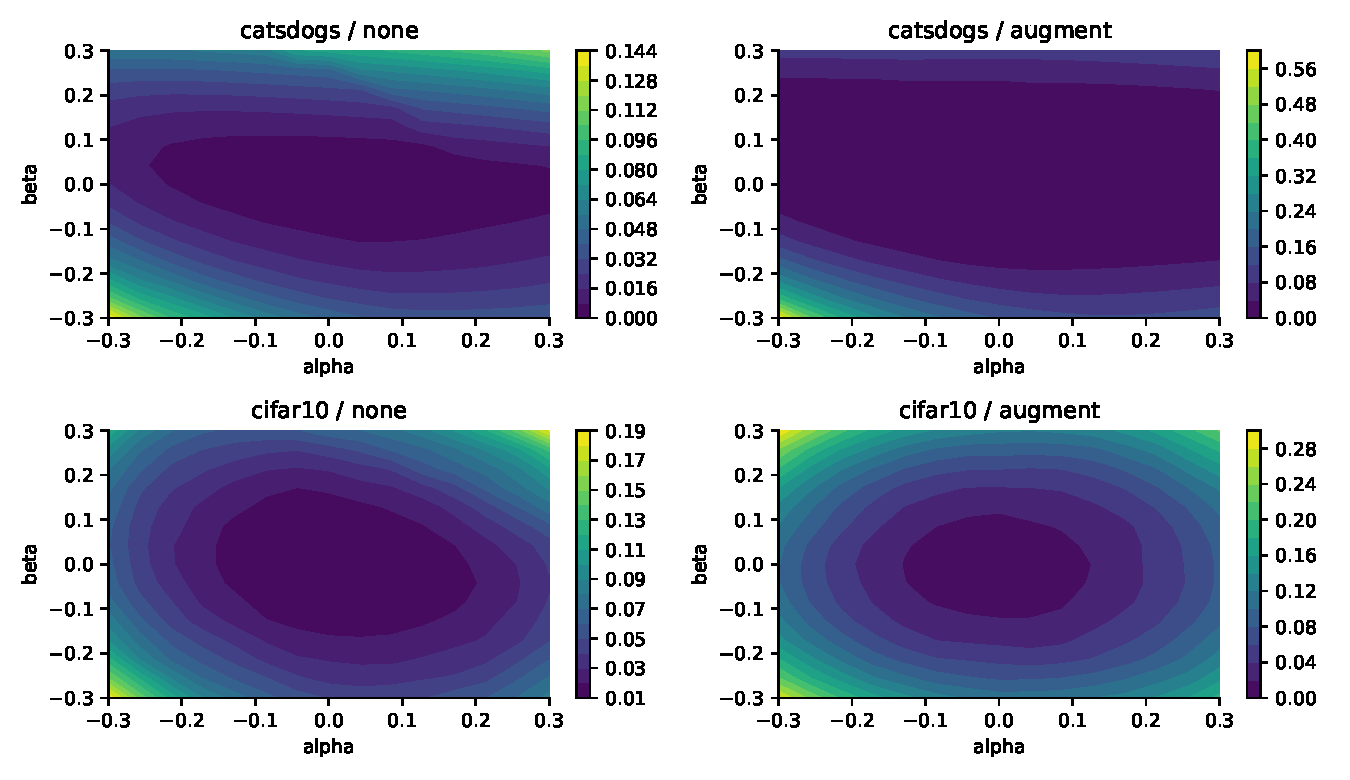
\includegraphics[width=.72\linewidth]{figures/landscape.pdf}\par\small Training BCE slices for seed-17 clean width-4 trees, direction pair 0. Colour scales differ; read their numeric bars. All three direction pairs and decision-flip maps are supplied.\end{center}
Directions are normalized per weight row, inspired by normalized landscape visualizations~\cite{li}; biases and correction coefficients are held fixed. Hard decisions are recomputed. Diagnostic loss is unweighted root-output BCE, not local balanced BCE or multiclass softmax test loss. Samples and views are fixed within each slice; augmented and unaugmented training subsets are not identical view collections. To quantify sharpness, the table gives the mean BCE rise above the centre in annuli of radius $0.1,0.2,0.3$ (width $\pm0.05$), averaged over the three direction pairs. At radius 0.3 augmented fits rise about 2--3 times more than unaugmented ones (for example training BCE $+0.098$ versus $+0.042$ on CIFAR-10), so these sampled directions do not support a simple ``augmentation flattens the minimum'' explanation. This is one seed and one width, and the augmented training set differs from the unaugmented one. Neither the slices nor the conditional Hessians establish global flatness or causality.
\begin{center}\small\begin{tabular}{llrrrrrr}\toprule
 & & \multicolumn{3}{c}{Training BCE rise} & \multicolumn{3}{c}{Validation BCE rise}\\
Dataset & Fit & 0.1 & 0.2 & 0.3 & 0.1 & 0.2 & 0.3\\\midrule
Cats vs Dogs & none & 0.0024 & 0.0093 & 0.0223 & 0.0082 & 0.0156 & 0.0306\\
 & augment & 0.0005 & 0.0114 & 0.0519 & 0.0124 & 0.0453 & 0.0980\\
CIFAR-10 & none & 0.0032 & 0.0157 & 0.0422 & 0.0016 & 0.0151 & 0.0416\\
 & augment & 0.0087 & 0.0381 & 0.0979 & 0.0113 & 0.0396 & 0.0930\\\bottomrule
\end{tabular}\end{center}

\section{Conclusions, limitations and reproducibility}
\textbf{Augmentation and fitting.} Finite input augmentation is compatible with interpolation and, in the clean 25\%-pool root-only comparison, lowers test error by 0.15--0.50 points at widths 32 and 256 where the four-copies control does not (Section 3). Under 15\% label noise it is harmful at small and medium widths (+1.8 to +5.9 points) and helps only at the largest widths, by under 0.6 points. Clean matched capacity comparisons and final ensemble comparisons provide complementary evidence.

\textbf{Ensembles.} Hard voting improves over average individual members in these experiments. The primary augmented-versus-unaugmented seven-member comparison supports a CIFAR-10 gain; Cats vs Dogs remains statistically inconclusive under the paired image bootstrap. The CIFAR-10 gain comes mainly from stronger augmented members and fewer shared errors, not from higher disagreement, and the ensembles do not beat a wider single tree from the earlier assignment. Diverse banks do not imply independent errors, because all members share the dataset and pretrained representation.

\textbf{Bias--variance and landscape.} More samples generally help CIFAR-10 in this grid, while increased epoch budgets raise prediction variance and replicate decision disagreement. Cats vs Dogs shows exceptions to monotonic sample-size effects. In sampled directions augmented fits rise more steeply (about 2--3 times at radius 0.3), so augmentation did not flatten the minimum here. Conditional readout convexity coexists with a nonconvex, hard-decision tree. A good test score cannot be inferred from a two-dimensional landscape alone.

\textbf{Innovations and interpretation.} The controlled diverse-bank ensemble and the persistence-weighted correction rule are the proposed experimental contributions. The latter fails to establish a meaningful improvement, suggesting that persistent errors are not necessarily the most useful errors to emphasize. A further insight is that increasing node width can remove the need for children, so the resulting topology must be reported when discussing capacity or size. The shared frozen trunk keeps ensembles relatively compact, but also limits representation diversity.

\textbf{Future work.} Use fresh external test data, more data/initialization seeds and repeated independent committees, including interpolating (wide-root) committees and parameter-matched single-tree baselines; test inverse persistence weighting under label noise; test online augmentation and compute-matched controls; investigate correction depth and width jointly; assess calibration separately from accuracy; test wider or differently regularized noisy models under a new validation protocol. These are future experiments, not reasons to retune against the test scores reported here. A larger balanced augmentation audit would cover every CIFAR class and quantify crop failures.

\textbf{Reproducibility and code.} The \texttt{continuation/} folder of the repository contains the training source, plans, per-run records, analysis outputs, an ensemble check script, figures and this LaTeX source. Original numerical feature banks and model checkpoints remain on my Mac; preserve them for inference reproduction. The source snapshot preserves the training modules used for the runs. The final analysis removes duplicate configurations when calculating seed spread. The report can be compiled with two calls to \texttt{pdflatex Tree\_Continuation\_Report.tex} from its report directory.

The Assignment 4 code is in the root of the repository listed above; the continuation code, plans, run records, analysis outputs and this report are in its \texttt{continuation/} folder. Feature banks and model checkpoints are too large for the repository and are kept locally.

\begin{center}\small\begin{tabular}{p{48mm}p{103mm}}\toprule
Assignment requirement & Evidence in this report\\\midrule
Augmentation + overfitting + double descent & Section 3: fitted error and test width curves; Section 6: actual epoch trajectories; negative findings explicit.\\
Multiple trees and majority voting & Section 4: complete predictors, committee-size curves, tie rule, matched primary comparison.\\
Bias/variance versus samples and epochs & Section 5: crossed repeats, exact empirical identity, sample sizes and per-node budgets.\\
Loss landscape & Section 6: three-direction slice experiment, hard decisions, conditional convexity and limits.\\
Innovation and supported conclusions & Sections 4 and 7: diversity and persistence ablations, uncertainty and future directions.\\\bottomrule
\end{tabular}\end{center}

\begin{thebibliography}{9}\small
\bibitem{nakkiran} P. Nakkiran et al. \emph{Deep Double Descent: Where Bigger Models and More Data Hurt}. ICLR, 2020. \url{https://arxiv.org/abs/1912.02292}.
\bibitem{yang} Z. Yang et al. \emph{Rethinking Bias-Variance Trade-off for Generalization of Neural Networks}. ICML, PMLR 119:10767--10777, 2020. \url{https://proceedings.mlr.press/v119/yang20j.html}.
\bibitem{li} H. Li et al. \emph{Visualizing the Loss Landscape of Neural Nets}. NeurIPS, 2018. \url{https://arxiv.org/abs/1712.09913}.
\end{thebibliography}
\end{document}
